\section{API Layer} 

\begin{frame}
    \frametitle{ Components}
    \begin{figure}
        \centering
        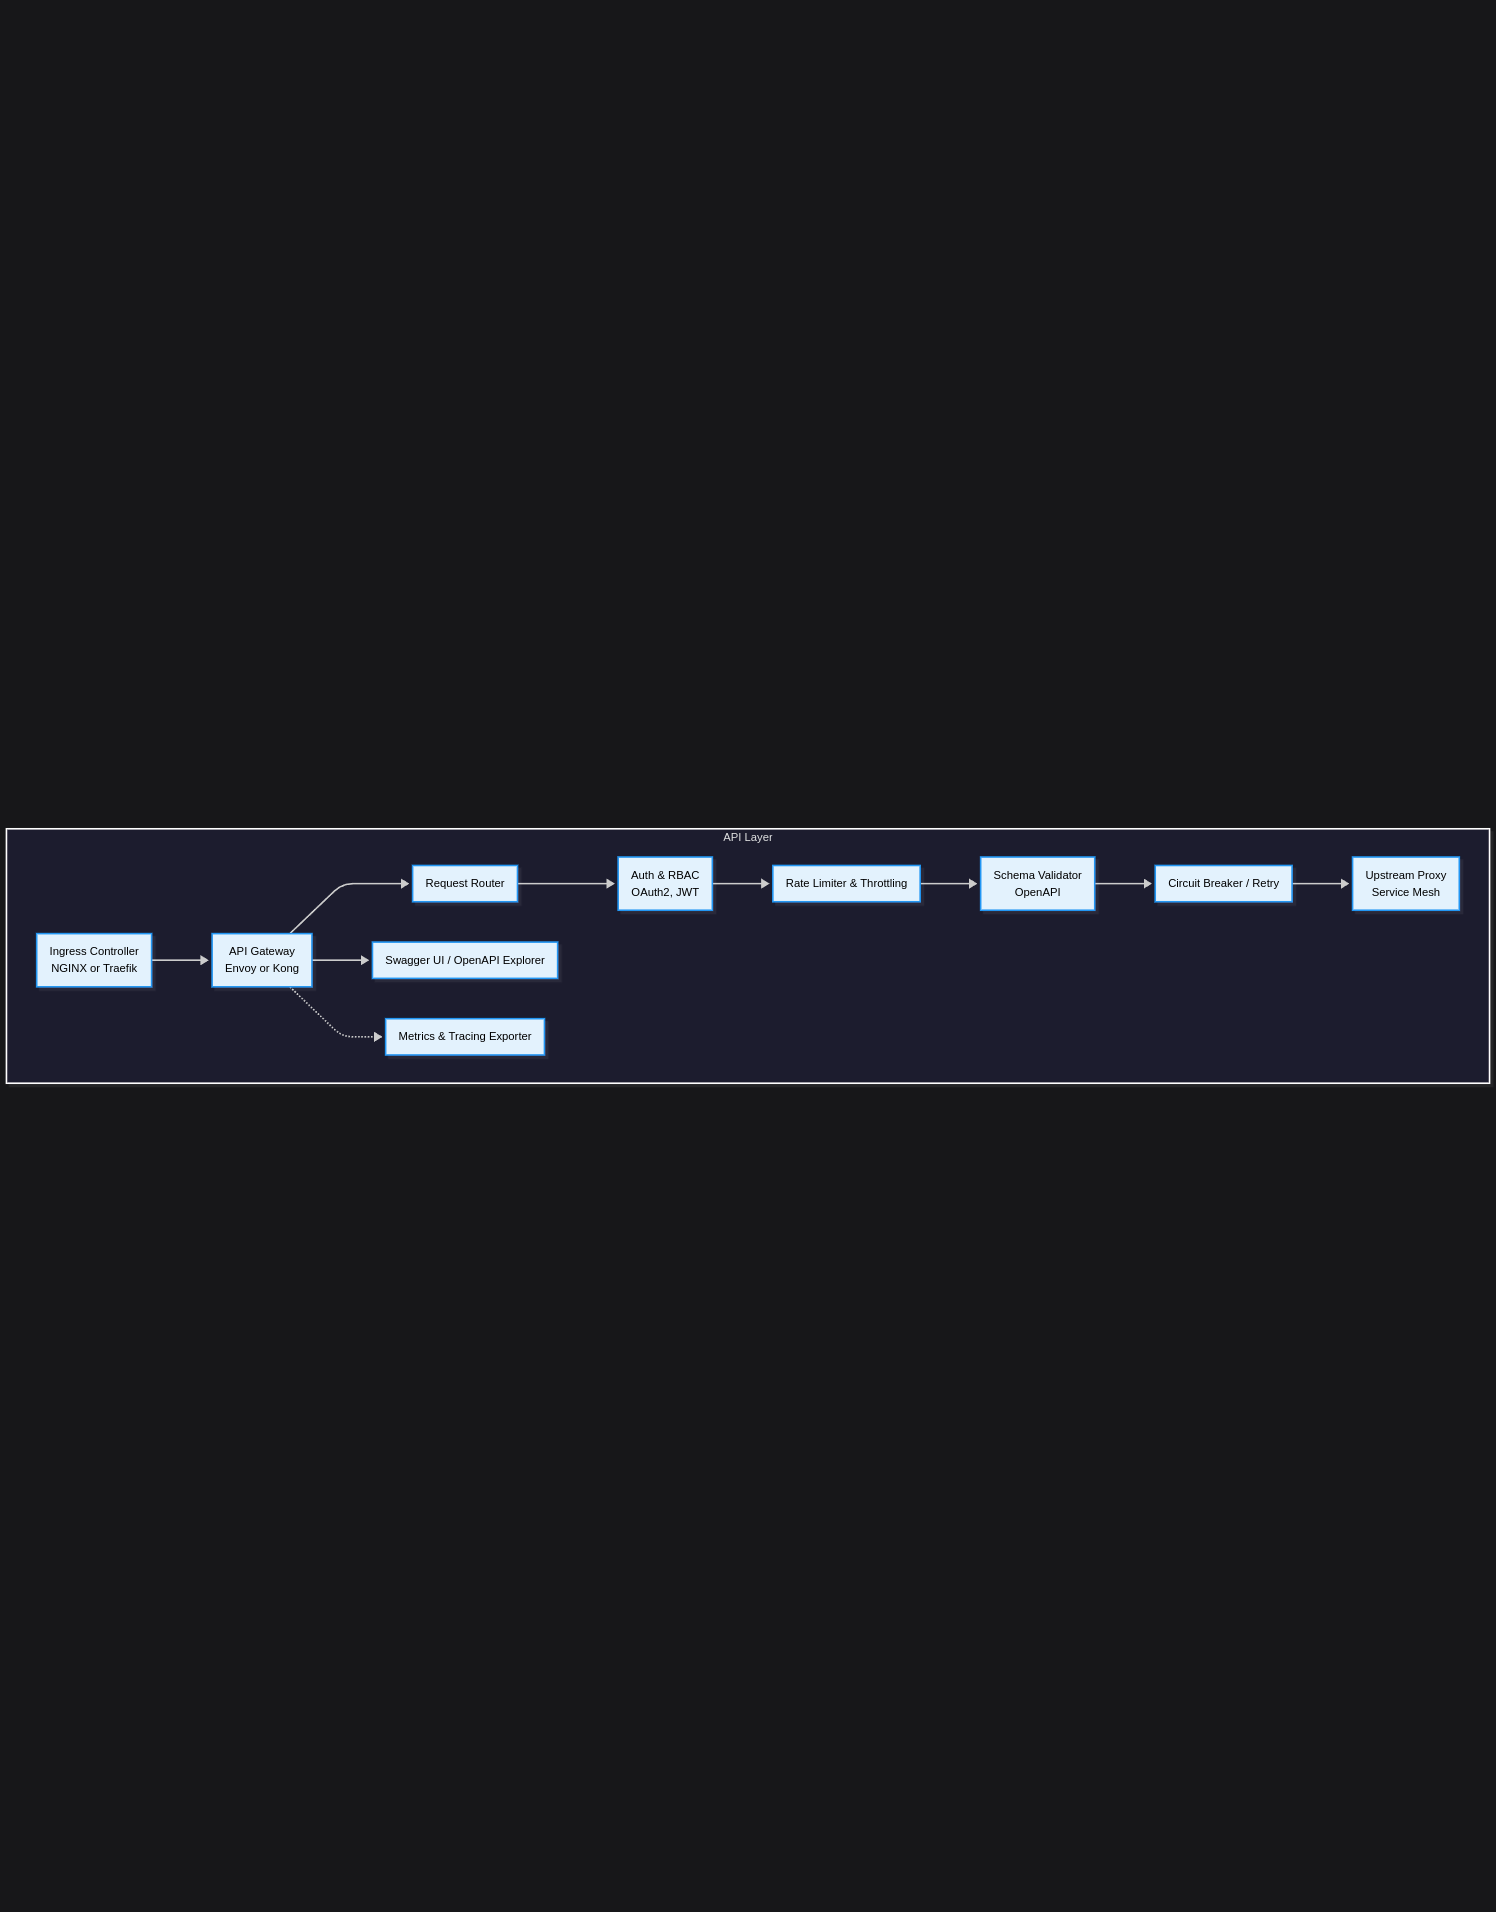
\includegraphics[width=0.8\textwidth]{api/layout.png} % Adjusted the scale of the image to 0.5
        \caption{Layout}
    \end{figure}
\end{frame}

\begin{frame}
    \frametitle{Sequence Flow}
    \begin{figure}
        \centering
        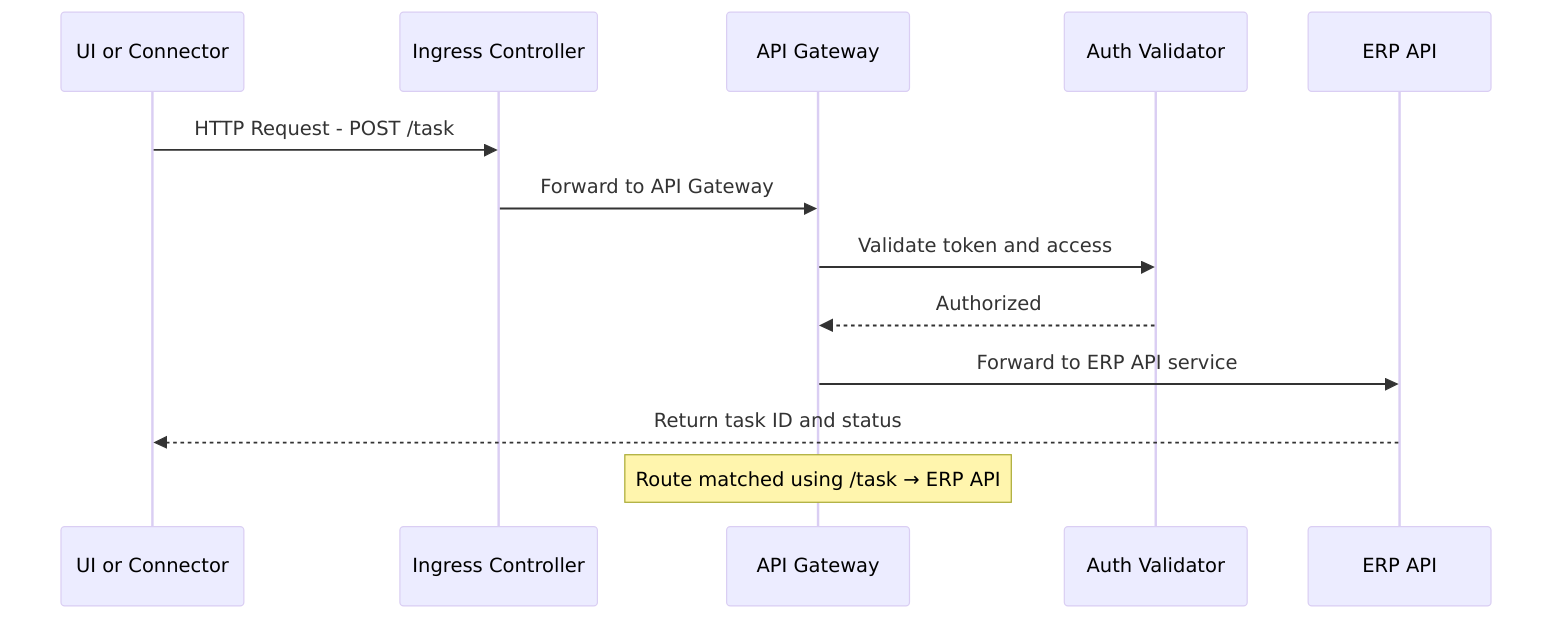
\includegraphics[width=0.8\textwidth]{api/sequence.png} % Adjusted the scale of the image to 0.5
        \caption{Sequence Flow}
    \end{figure}
\end{frame}

\begin{frame}
    \frametitle{Components}
    \begin{itemize}
        \item \textbf{Ingress Controller}: Terminate external traffic, route internal requests securely.
        \item \textbf{API Gateway}: Unified entry point for all internal APIs and services.
        \item \textbf{Auth Handler}: Validate tokens, enforce roles and access policies.
        \item \textbf{Rate Limiter}: Enforce request limits per user or project to protect backend.
        \item \textbf{Routing Layer}: Route requests to ERP, ETL, File, Agent, or Storage APIs.
        \item \textbf{ERP API}: Handles project creation, task status updates, SLA queries.
        \item \textbf{File API}: File upload, version fetch, document metadata access.
        \item \textbf{ETL API}: Start extraction jobs, monitor ETL status, retry failures.
        \item \textbf{Agent API}: Trigger agents, collect output, monitor agent health.
        \item \textbf{Storage API}: Access vector search, metadata store, audit logs.
    \end{itemize}
\end{frame}


% \begin{frame}
%     \frametitle{Technical Responsibilities - Part 1}
%     \begin{table}[h!]
% \centering
% \renewcommand{\arraystretch}{1.2}
% \begin{tabular}{|p{3cm}|p{7cm}|}
% \hline
% \textbf{Component} & \textbf{Technical Responsibility} \\
% \hline
% Ingress Controller & TLS termination, path routing to internal services \\
% \hline
% API Gateway & Implements OpenAPI spec routing, request logging, versioning \\
% \hline
% Auth Handler & OAuth or token-based validation, integrates with Vault or external IdP \\
% \hline
% Rate Limiter & Per-project or per-user limits using Redis or Kong plugin \\
% \hline
% Routing Layer & Load balances and forwards requests to correct internal microservice \\
% \hline
% ERP API & Built using REST or GraphQL, integrates with task DB and SLA tracker \\
% \hline
% \end{tabular}
% \caption{API Layer - Technical Responsibilities (Part 1)}
% \end{table}
% \end{frame}

% \begin{frame}
%     \frametitle{Technical Responsibilities - Part 2}
%     \begin{table}[h!]
% \centering
% \renewcommand{\arraystretch}{1.2}
% \begin{tabular}{|p{3cm}|p{7cm}|}
% \hline
% \textbf{Component} & \textbf{Technical Responsibility} \\
% \hline
% File API & Serves file IO endpoints, exposes version trees and document links \\
% \hline
% ETL API & Controls extract pipeline orchestration and logs \\
% \hline
% Agent API & Communicates with agent dispatcher, scaffold registry, and result handlers \\
% \hline
% Storage API & Exposes audit logs, vector search, and object metadata via internal endpoints \\
% \hline
% \end{tabular}
% \caption{API Layer - Technical Responsibilities (Part 2)}
% \end{table}
% \end{frame}